
\section{Approach}

Describe the final approach you are take for this problem.
For instance, here you would describe the details of the network’s
architecture. What training parameters and techniques you have used.
The computational complexity of your model. And similar questions.
To help explain your approach please make figures to accompany your
text description. (1-3 pages)

%Not sure these sections actually belong here do with them as you please
\subsection{Data Collection}
%not sure if this is actually something we want to include and if so where it should be introduced so feel free to change it
%TODO possibly add a reference instead of the hyperlink
During experimentation we mostly relied on the popular benchmark dataset \href{https://www.cs.toronto.edu/~kriz/cifar.html}{CIFAR-10}, however an additional data set was collected using \href{https://www.flickr.com/services/api/}{Flickr's API}. Due to varying amounts of quality pictures of objects that would be interesting to base the image generation on, a collection that included mostly different reptiles with a fair amount of arachnid's thrown into the mix was ultimately settled upon therefore this data set will be referred to as the Reptiles form here on. In total the data set is made up of approximately 20k color images all re-sized to dimensions of 108x108x3 before training was conducted. Examples of images can be seen in figure \ref{fig:reptiles}.

\begin{figure}[H]
\centering
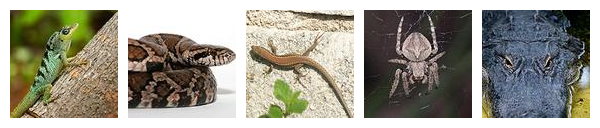
\includegraphics[width=\textwidth]{figures/reptiles.png}
\caption{Examples from the Reptiles data set}
\label{fig:reptiles}
\end{figure}




